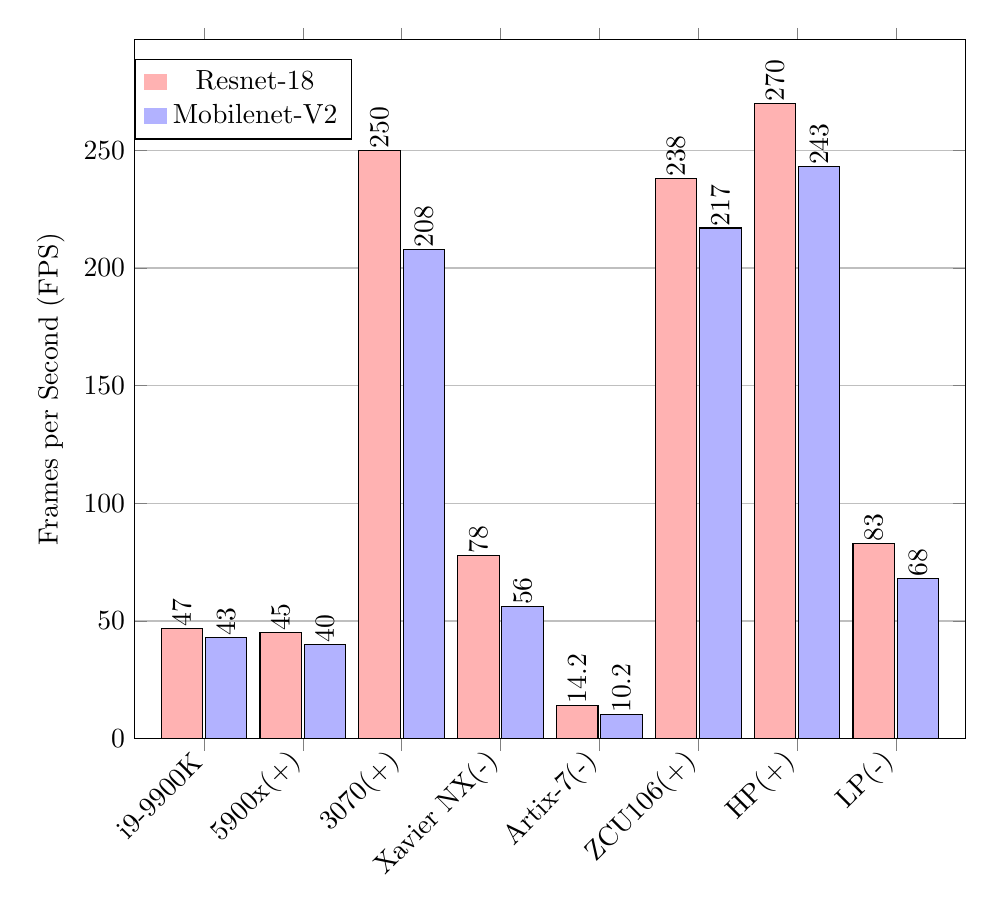
\begin{tikzpicture}
\pgfplotsset{width=\textwidth,compat=1.3}
\begin{axis}[
    legend style={},
    ybar=1pt,
    ymin=0,
    bar width =15pt,
    legend image code/.code={\draw[#1, draw=none] (0cm,-0.1cm) rectangle (0.3cm,0.1cm);
                },
    ymajorgrids = true,
    legend style={at={(-0.000001,0.915)},
                   anchor=west,legend columns=1},
    ylabel={Frames per Second (FPS)},
    symbolic x coords={i9-9900K, 5900x(+), 3070(+), Xavier NX(-), Artix-7(-), ZCU106(+), HP(+), LP(-)},
    xtick=data,
    nodes near coords,
    nodes near coords style={font=\medium, anchor=west,rotate=90,inner
    xsep=0.5pt},
    x tick label style = { rotate=45, anchor=east},
    xlabel style={font=\large},
    ]

\addplot [fill=red!30] coordinates {(i9-9900K, 47)(5900x(+), 45)(3070(+), 250)(Xavier NX(-), 78) (Artix-7(-), 14.2)(ZCU106(+), 238)(HP(+), 270)(LP(-), 83)};%Resnet

\addplot [fill=blue!30]  coordinates {(i9-9900K, 43)(5900x(+), 40)(3070(+), 208)(Xavier NX(-), 56) (Artix-7(-), 10.2)(ZCU106(+), 217)(HP(+), 243)(LP(-), 68) };%Mobilenet

\legend{Resnet-18,Mobilenet-V2}
\end{axis}
\end{tikzpicture}
